% Use xelatex to generate pdf file of this presentation

\documentclass[xcolor=table]{beamer}
\usepackage{roboto}
\usepackage[russian]{babel}
\usetheme{Copenhagen}

% Simple way to put a code listing to the slide
\usepackage{listings}

% Tabular-specific packages
\usepackage{makecell}
\usepackage{tabu, booktabs}

\usepackage[symbol*]{footmisc}
\setfnsymbol{wiley}

\usepackage{tikz}
\usepackage{graphicx}
  \logo{
\includegraphics[scale=0.1]{pics/PostgresPro_logo}}
%Information to be included in the title page:
\title{pg\_index\_stats}
\subtitle{manage\ extended\ statistics\ automatically}
\author{\underline{Lepikhov A.}, Rybakina A.}
\institute{Postgres Professional}
%\titlegraphic{\includegraphics[scale=0.05]{project_url}}
\date{2024}

% Add page numbers in footnote
\expandafter\def\expandafter\insertshorttitle\expandafter{%
  \insertshorttitle\hfill%
  \insertframenumber\,/\,\inserttotalframenumber}

% Custom commands
\newcommand{\tbltext}[1]{\ttfamily\footnotesize#1}

% Custom colours: https://latexcolor.com
\definecolor{armygreen}{rgb}{0.29, 0.33, 0.13}
\definecolor{darkgreen}{rgb}{0.0, 0.5, 0.0}
\definecolor{lightlightgray}{gray}{0.9}

% -----------------------------

\begin{document}

\begin{frame}
\titlepage
   \tikz [remember picture,overlay]
    \node at
        ([yshift=2.0cm, xshift=-4.8cm]current page.center) 
        {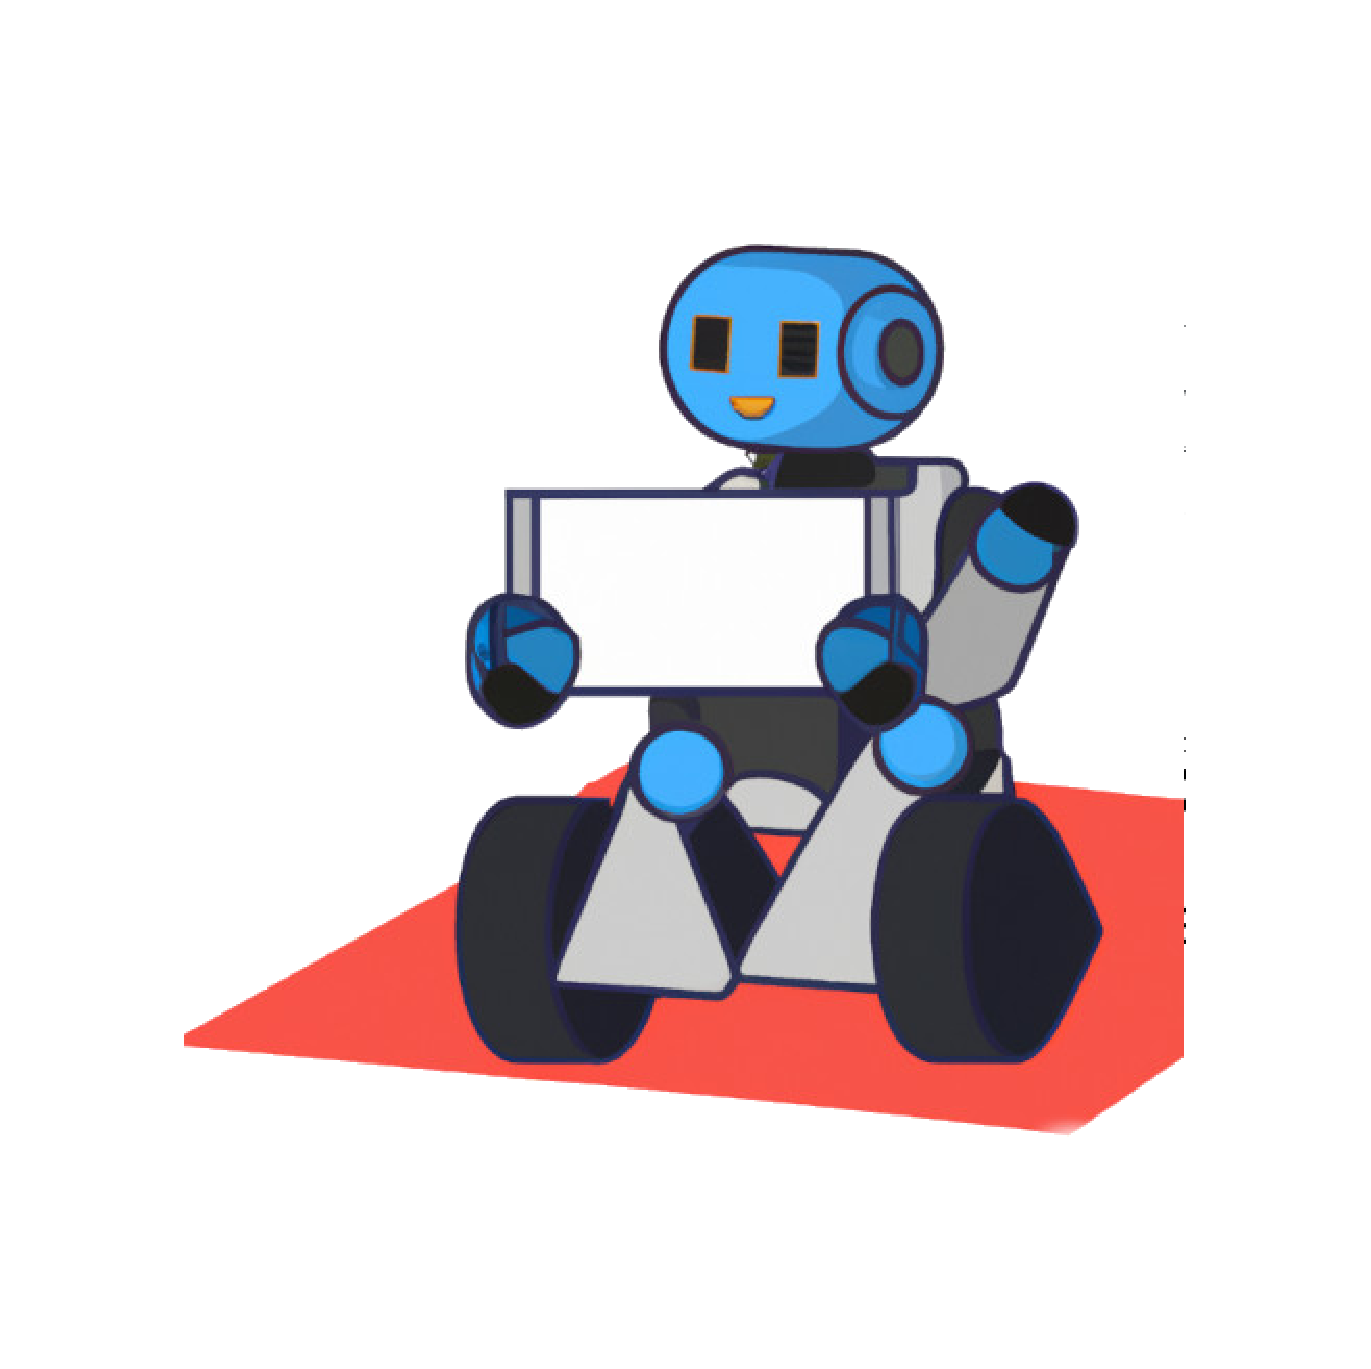
\includegraphics[scale=0.05]{pics/project_logo}};

\end{frame}


\begin{frame}[fragile]\frametitle{Self Introduction}
\begin{columns}\begin{column}{0.6\textwidth}
\begin{itemize}
  \item Core Developer in Postgres Professional since 2017.
  \item Contributing to the PostgreSQL project since 2017:\\ \textit{Self-Join Elimination, GROUP-BY optimisation, OR <-> ANY transformation}.
  \item Ph.D. in Computer Sciences (Distributed Databases), MSU, 2008.
  \item Designed extensions: AQO, sr\_plan, pg\_index\_stats ...
\end{itemize}
\end{column}
\begin{column}{0.4\textwidth}
  \includegraphics[scale=0.05]{pics/selfie}
\end{column}\end{columns}
\end{frame}


\begin{frame}[fragile]\frametitle{Quick start}
\lstset{language=sql, frame=none, tabsize=2, identifierstyle=\color{black},
  backgroundcolor=\color{lightlightgray},
  keywordstyle=\bfseries\color{green!40!black},showspaces=false, showtabs=false, showstringspaces=false}
\begin{lstlisting}[basicstyle=\footnotesize]
CREATE EXTENSION 'pg_index_stats';
CREATE TABLE test (x int,y int,z text);
CREATE INDEX ON test (x,y);
CREATE INDEX ON test (z,y);
\dX
\end{lstlisting}
\begin{lstlisting}[basicstyle=\tiny]
                         List of extended statistics
 Schema |     Name      |   Definition   | Ndistinct | Dependencies |   MCV   
--------+---------------+----------------+-----------+--------------+---------
 public | test_x_y_stat | x, y FROM test | defined   | defined      | defined
 public | test_z_y_stat | y, z FROM test | defined   | defined      | defined
\end{lstlisting}
\end{frame}

\begin{frame}[fragile]\frametitle{Quick start - II}
\lstset{language=sql, frame=none, tabsize=2, identifierstyle=\color{black},
  backgroundcolor=\color{lightlightgray},
  keywordstyle=\bfseries\color{green!40!black},showspaces=false, showtabs=false, showstringspaces=false}
\begin{lstlisting}[basicstyle=\footnotesize]
DROP INDEX test_x_y_idx;
\end{lstlisting}
\begin{lstlisting}[basicstyle=\tiny]
                         List of extended statistics
 Schema |     Name      |   Definition   | Ndistinct | Dependencies |   MCV   
--------+---------------+----------------+-----------+--------------+---------
 public | test_z_y_stat | y, z FROM test | defined   | defined      | defined
\end{lstlisting}
\end{frame}


\begin{frame}[fragile]\frametitle{GUCs \& Funcs}
\begin{itemize}
  \item \textit{mode} - disabled | all | univariate | multivariate
  \item \textit{columns\_limit}
  \item \textit{pg\_index\_stats\_build(relname, mode)}
  \item \textit{pg\_index\_stats\_rebuild()}
  \item \textit{pg\_index\_stats\_remove()}
\end{itemize}
\end{frame}

\begin{frame}[fragile]\frametitle{Short Tech Backtrack}
Two-step process:
\begin{itemize}
  \item Object Access Hook - gather candidate OIDs 
  \item Utility Hook - create extended statistics after a successful utility statement
\end{itemize}
Set dependency of auto-generated statistics on the extension and index relation.\\
Add specific description for auto-generated statistics
\end{frame}

\begin{frame}[fragile]\frametitle{What is the reason?}
	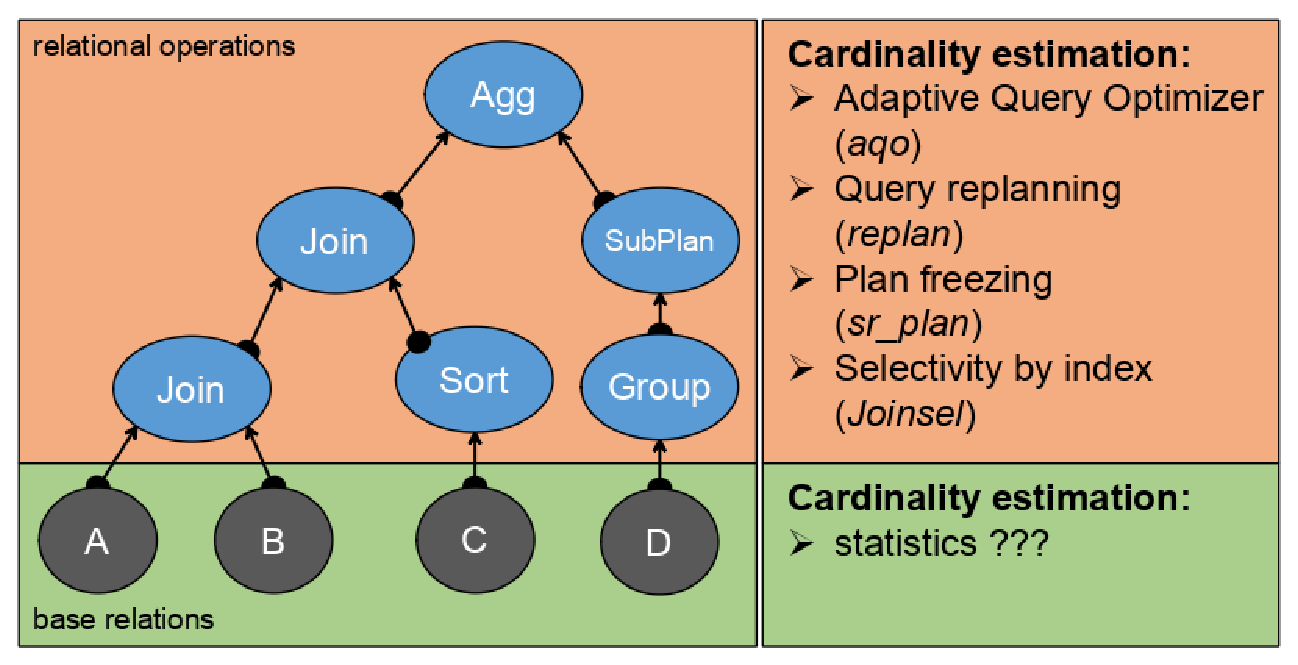
\includegraphics[scale=0.52]{pics/querytree}
\end{frame}

\begin{frame}[fragile]\frametitle{Query auto-generation frameworks}
\begin{center}
	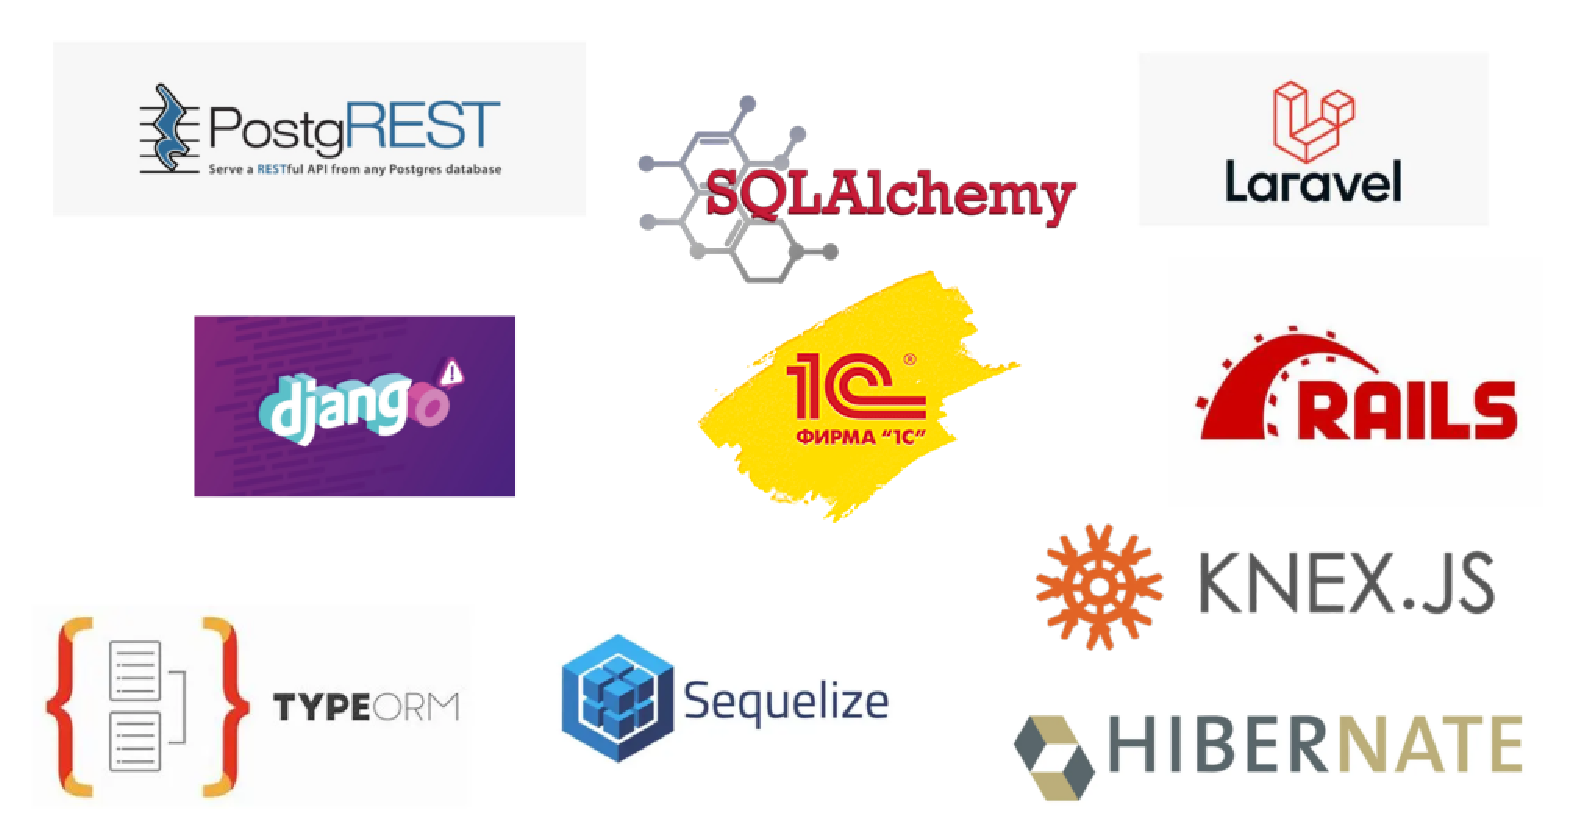
\includegraphics[scale=0.4]{pics/orms}
\end{center}
\end{frame}

\begin{frame}[fragile]\frametitle{Redundant expressions}
\lstset{language=sql, frame=none, tabsize=2, identifierstyle=\color{black},
  backgroundcolor=\color{white},
  keywordstyle=\bfseries\color{green!40!black},showspaces=false, showtabs=false, showstringspaces=false}
\begin{center}
\begin{tabular}{|l|c|c|}
	\hline
	% Header
	\multicolumn{1}{|c|}{Query} & Planned rows & Actual rows \\
	\hline
\begin{lstlisting}[basicstyle=\footnotesize]
SELECT * FROM power_plants
WHERE
  country = 'RUS';
\end{lstlisting}
& \cellcolor{green}544 & \cellcolor{green}544 \\
	\hline
\begin{lstlisting}[basicstyle=\footnotesize]
SELECT * FROM power_plants
WHERE
  country = 'RUS' AND
  country_long = 'Russia';
\end{lstlisting}
& \cellcolor{red}8 & \cellcolor{green}544 \\
	\hline
\end{tabular}
\footnotetext{
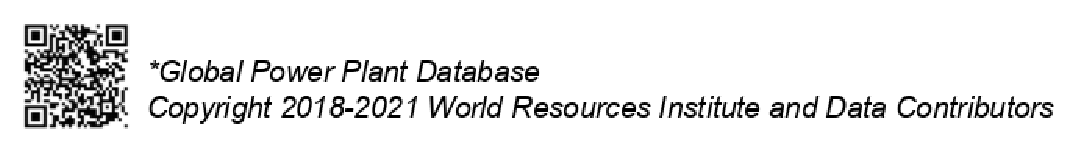
\includegraphics[scale=0.4]{pics/GPPD-copyright}
}
\end{center}
\end{frame}

% %%%%%%%%%%%%%%%%%%%%%%%%%%%%%%%%%%%%%%%%%%%%%%%%%%%%%
%
% The main question that should be explained.
%
% %%%%%%%%%%%%%%%%%%%%%%%%%%%%%%%%%%%%%%%%%%%%%%%%%%%%%
\begin{frame}[fragile]\frametitle{The question}
\begin{quote}
Why can database systems, which manage all the data, not analyse it and find at least in-table dependencies and interconnections?
\end{quote}
\end{frame}

% %%%%%%%%%%%%%%%%%%%%%%%%%%%%%%%%%%%%%%%%%%%%%%%%%%%%%
%
% Rationale for the usage of indexes. An example.
%
% %%%%%%%%%%%%%%%%%%%%%%%%%%%%%%%%%%%%%%%%%%%%%%%%%%%%%
\begin{frame}[fragile]\frametitle{Why indexes?}
\begin{lstlisting}[basicstyle=\footnotesize]
Table "Parcels":
Indexes:
    "parcel_pkey" PRIMARY KEY, btree (id)
    "parcel_parcel_id" btree (parcel_id)
    "parcel_id_prik" btree (parcel_id, prik)
    "parcel_id_sn_pol" btree (parcel_id, sn_pol)
    "parcel_par_begin" btree (parcel_id, prik_begin_period)
    "parcel_par_patient" btree (parcel_id, patient_id)
    "parcel_par_recid" btree (parcel_id, recid)
    "parcel_per_prik" btree (period, prik)
\end{lstlisting}
\end{frame}

\lstset{language=sql, frame=none, tabsize=2, identifierstyle=\color{black},
  backgroundcolor=\color{white}, showspaces=false, showtabs=false, showstringspaces=false,
  columns=fullflexible, % Restore default spaces between letters
  basicstyle=\rmfamily\scriptsize,
  stringstyle=\color{purple},
  keywordstyle=\bfseries\color{green!40!black},
  numberstyle=\tiny\color{gray}}
  
% %%%%%%%%%%%%%%%%%%%%%%%%%%%%%%%%%%%%%%%%%%%%%%%%%%%%%
%
% How extended statistics helps
%
% %%%%%%%%%%%%%%%%%%%%%%%%%%%%%%%%%%%%%%%%%%%%%%%%%%%%%
\begin{frame}[fragile]\frametitle{Extended v/s Plain Statistics}
SELECT * FROM power\_plants WHERE ...
\begin{center}
\begin{tabular}{|l|c|c|c|}
	\hline
	% Header
	\multicolumn{1}{|c|}{\tbltext{Query}} & \tbltext{\makecell{Plain\\ stat}} & \tbltext{\makecell{Extended\\ stat}} & \tbltext{\makecell{Actual\\ rows}} \\
	\hline
\begin{lstlisting}
country = 'RUS';
\end{lstlisting}
& \cellcolor{green}544 & \cellcolor{green}545 & \cellcolor{green}544 \\
	\hline
\begin{lstlisting}
AND primary_fuel IN ('Solar')
\end{lstlisting}
& \cellcolor{darkgreen}166 & \cellcolor{green}57 & \cellcolor{green}57 \\
	\hline
\begin{lstlisting}
primary_fuel IN
  ('Solar', 'Biomass')
\end{lstlisting}
& \cellcolor{darkgreen}189 & \cellcolor{green}60 & \cellcolor{green}60 \\
	\hline
\begin{lstlisting}
primary_fuel IN
  ('Solar', 'Biomass', 'Coal')
\end{lstlisting}
& \cellcolor{darkgreen}225 & \cellcolor{green}156 & \cellcolor{green}156 \\
	\hline
\begin{lstlisting}
AND source = 'Wiki-Solar'
\end{lstlisting}
& \cellcolor{red}24 & \cellcolor{green}46 & \cellcolor{green}40 \\
	\hline
\begin{lstlisting}
AND longitude > 40.
AND longitude < 70.
\end{lstlisting}
& \cellcolor{red}1 & \cellcolor{red}1 & \cellcolor{green}33 \\
	\hline
\end{tabular}
\footnotetext{
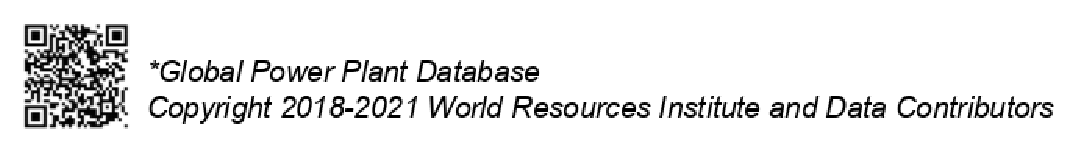
\includegraphics[scale=0.4]{pics/GPPD-copyright}
}
\end{center}
\end{frame}

% %%%%%%%%%%%%%%%%%%%%%%%%%%%%%%%%%%%%%%%%%%%%%%%%%%%%%
%
% Why do we need a multicolumn histogram
%
% %%%%%%%%%%%%%%%%%%%%%%%%%%%%%%%%%%%%%%%%%%%%%%%%%%%%%
\begin{frame}[fragile]\frametitle{Does multicolumn histogram make sense?}
\begin{center}
	
\end{center}
\end{frame}

% %%%%%%%%%%%%%%%%%%%%%%%%%%%%%%%%%%%%%%%%%%%%%%%%%%%%%
%
% Extended statistics v/s histogram
%
% %%%%%%%%%%%%%%%%%%%%%%%%%%%%%%%%%%%%%%%%%%%%%%%%%%%%%
\begin{frame}[fragile]\frametitle{Multicolumn histogram advantage}
SELECT * FROM power\_plants WHERE ...
\begin{center}
\begin{tabular}{|l|c|c|c|c|}
	\hline
	% Header
	\multicolumn{1}{|c|}{\tbltext{Query}} & \tbltext{\makecell{Plain\\ stat}} & \tbltext{\makecell{Extended\\ stat}} & \tbltext{Histogram} & \tbltext{\makecell{Actual\\ rows}} \\
	\hline
\begin{lstlisting}
country = 'RUS';
\end{lstlisting}
& \cellcolor{green}544 & \cellcolor{green}545 & \cellcolor{green}544 & \cellcolor{green}544 \\
	\hline
\begin{lstlisting}
AND primary_fuel IN ('Solar')
\end{lstlisting}
& \cellcolor{darkgreen}166 & \cellcolor{green}57 & \cellcolor{green}57 & \cellcolor{green}57 \\
	\hline
\begin{lstlisting}
primary_fuel IN
  ('Solar', 'Biomass')
\end{lstlisting}
& \cellcolor{darkgreen}189 & \cellcolor{green}60 & \cellcolor{green}60 & \cellcolor{green}60 \\
	\hline
\begin{lstlisting}
primary_fuel IN
  ('Solar', 'Biomass', 'Coal')
\end{lstlisting}
& \cellcolor{darkgreen}225 & \cellcolor{green}156 & \cellcolor{green}156 & \cellcolor{green}156 \\
	\hline
\begin{lstlisting}
AND source = 'Wiki-Solar'
\end{lstlisting}
& \cellcolor{red}24 & \cellcolor{green}46 & \cellcolor{green}42 & \cellcolor{green}40 \\
	\hline
\begin{lstlisting}
AND longitude > 40.
AND longitude < 70.
\end{lstlisting}
& \cellcolor{red}1 & \cellcolor{red}1 & \cellcolor{green}35 & \cellcolor{green}33 \\
	\hline
\end{tabular}
\footnotetext{
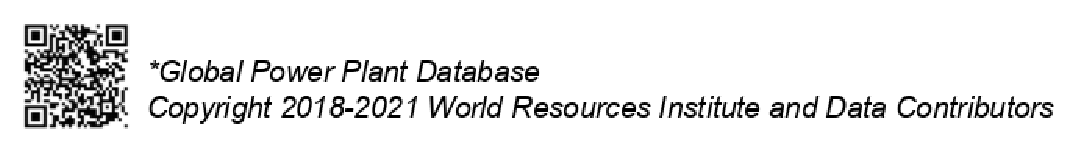
\includegraphics[scale=0.4]{pics/GPPD-copyright}
}
\end{center}
\end{frame}

% %%%%%%%%%%%%%%%%%%%%%%%%%%%%%%%%%%%%%%%%%%%%%%%%%%%%%
%
% Final frame
%
% %%%%%%%%%%%%%%%%%%%%%%%%%%%%%%%%%%%%%%%%%%%%%%%%%%%%%
\begin{frame}
\begin{center}
\begin{center}
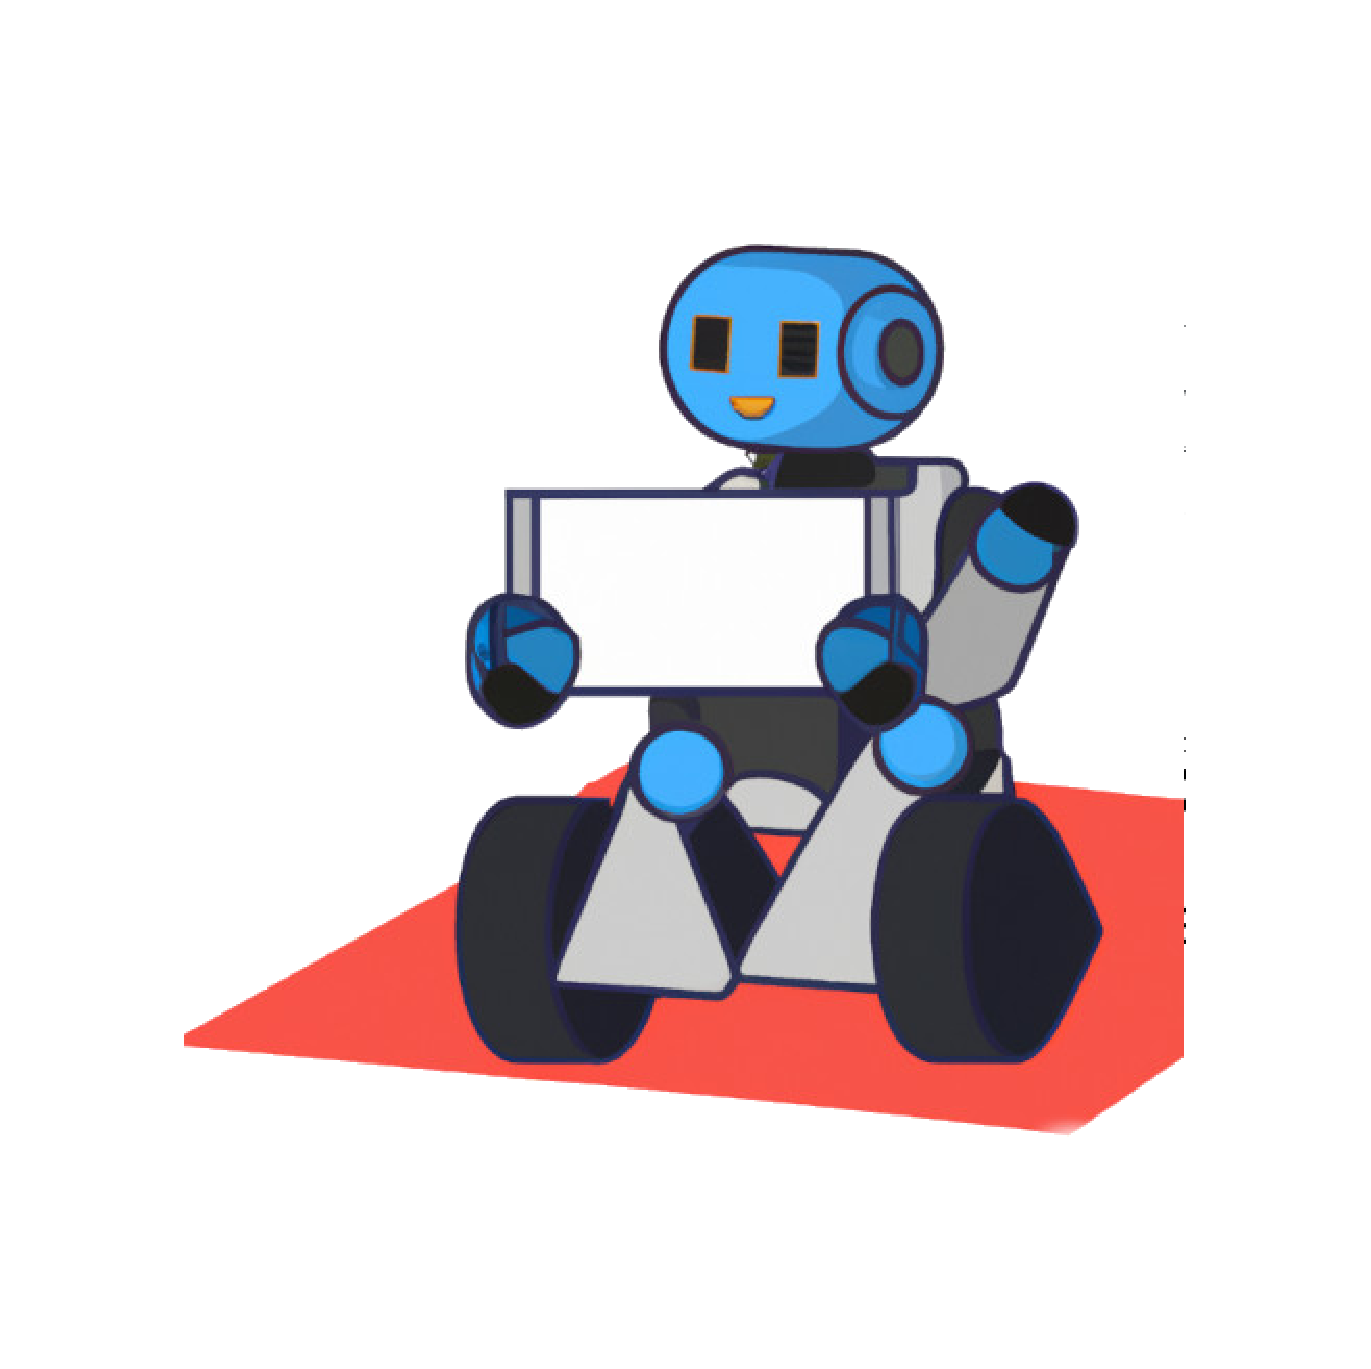
\includegraphics[scale=0.1]{pics/project_logo}
\end{center}
\huge{Questions ?}
\end{center}
\vspace{10pt}
\begin{center}
\begin{tabular}{rl}
\makecell[c]{
\includegraphics[scale=0.1]{pics/extensionlink}} & \tbltext{\makecell[l]{The pg\_index\_stats extension\\ github link}} \\
\makecell[c]{
\includegraphics[scale=0.1]{pics/pgpro}} & \tbltext{\makecell[l]{Postgres Professional LLC\\ The Russian Postgres Company}} \\
\end{tabular}
\end{center}
\end{frame}

\end{document}
